% This file was created with tikzplotlib v0.10.1.post5.
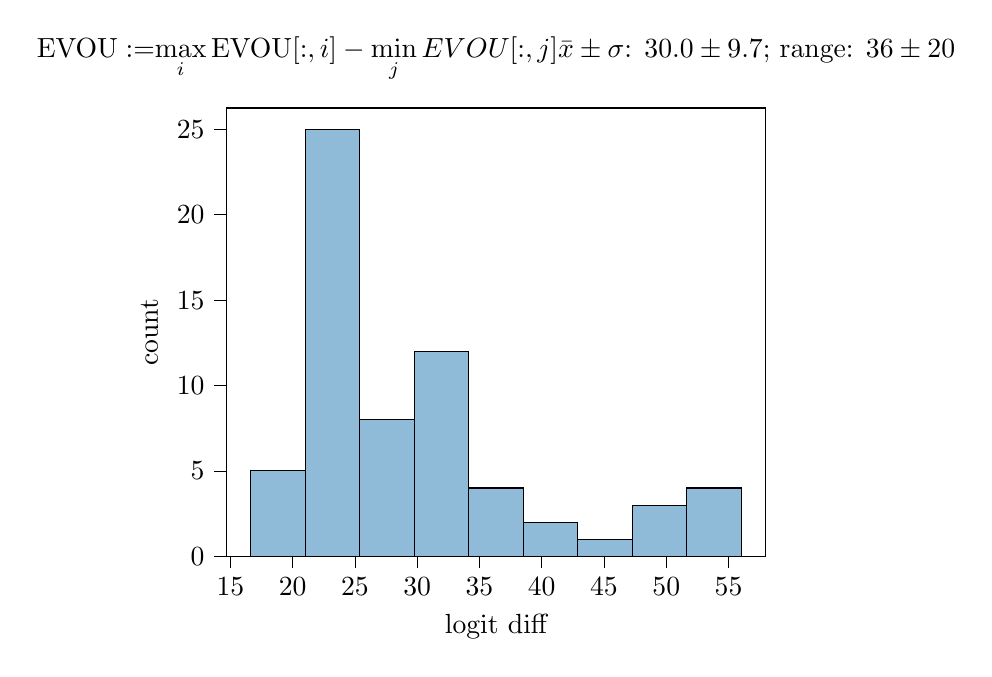
\begin{tikzpicture}

\definecolor{darkgray176}{RGB}{176,176,176}
\definecolor{steelblue31119180}{RGB}{31,119,180}

\begin{axis}[
tick align=outside,
tick pos=left,
title={\(\displaystyle \mathrm{EVOU} := \WE \WV \WO\WU \)\\
\(\displaystyle \max_i\mathrm{EVOU}[:,i] - \min_jEVOU[:,j]\)\\
\(\displaystyle \bar{x}\pm\sigma\): \(\displaystyle 30.0 \pm 9.7\); range: \(\displaystyle 36 \pm 20\)},
x grid style={darkgray176},
xlabel={logit diff},
xmin=14.6620410919189, xmax=57.9945064544678,
xtick style={color=black},
xtick={10,15,20,25,30,35,40,45,50,55,60},
xticklabels={
  \(\displaystyle {10}\),
  \(\displaystyle {15}\),
  \(\displaystyle {20}\),
  \(\displaystyle {25}\),
  \(\displaystyle {30}\),
  \(\displaystyle {35}\),
  \(\displaystyle {40}\),
  \(\displaystyle {45}\),
  \(\displaystyle {50}\),
  \(\displaystyle {55}\),
  \(\displaystyle {60}\)
},
y grid style={darkgray176},
ylabel={count},
ymin=0, ymax=26.25,
ytick style={color=black},
ytick={0,5,10,15,20,25,30},
yticklabels={
  \(\displaystyle {0}\),
  \(\displaystyle {5}\),
  \(\displaystyle {10}\),
  \(\displaystyle {15}\),
  \(\displaystyle {20}\),
  \(\displaystyle {25}\),
  \(\displaystyle {30}\)
}
]
\draw[draw=black,fill=steelblue31119180,fill opacity=0.5] (axis cs:16.6316986083984,0) rectangle (axis cs:21.0087153116862,5);
\draw[draw=black,fill=steelblue31119180,fill opacity=0.5] (axis cs:21.0087153116862,0) rectangle (axis cs:25.385732014974,25);
\draw[draw=black,fill=steelblue31119180,fill opacity=0.5] (axis cs:25.385732014974,0) rectangle (axis cs:29.7627487182617,8);
\draw[draw=black,fill=steelblue31119180,fill opacity=0.5] (axis cs:29.7627487182617,0) rectangle (axis cs:34.1397654215495,12);
\draw[draw=black,fill=steelblue31119180,fill opacity=0.5] (axis cs:34.1397654215495,0) rectangle (axis cs:38.5167821248372,4);
\draw[draw=black,fill=steelblue31119180,fill opacity=0.5] (axis cs:38.5167821248372,0) rectangle (axis cs:42.893798828125,2);
\draw[draw=black,fill=steelblue31119180,fill opacity=0.5] (axis cs:42.893798828125,0) rectangle (axis cs:47.2708155314128,1);
\draw[draw=black,fill=steelblue31119180,fill opacity=0.5] (axis cs:47.2708155314128,0) rectangle (axis cs:51.6478322347005,3);
\draw[draw=black,fill=steelblue31119180,fill opacity=0.5] (axis cs:51.6478322347005,0) rectangle (axis cs:56.0248489379883,4);
\end{axis}

\end{tikzpicture}
